\documentclass[conference]{IEEEtran}

\usepackage[T1]{fontenc}
\usepackage[utf8]{inputenc}
\usepackage{textcomp}

% Pandoc may emit some Unicode punctuation/symbols directly. Map common ones for pdflatex.
\DeclareUnicodeCharacter{00B0}{\textdegree}
\DeclareUnicodeCharacter{00B2}{\textsuperscript{2}}
\DeclareUnicodeCharacter{00D7}{\ensuremath{\times}}
\DeclareUnicodeCharacter{0394}{\ensuremath{\Delta}}
\DeclareUnicodeCharacter{2013}{--}
\DeclareUnicodeCharacter{2019}{'}
\DeclareUnicodeCharacter{201C}{``}
\DeclareUnicodeCharacter{201D}{''}
\DeclareUnicodeCharacter{2192}{\ensuremath{\rightarrow}}
\DeclareUnicodeCharacter{21D2}{\ensuremath{\Rightarrow}}
\DeclareUnicodeCharacter{2248}{\ensuremath{\approx}}

\usepackage{amsmath,amssymb}
\usepackage{graphicx}
\setkeys{Gin}{width=\linewidth,height=0.9\textheight,keepaspectratio}
\usepackage{booktabs}
\usepackage{longtable}
% Pandoc emits longtable which is incompatible with two-column mode.
% Add a post-processing step in build_paper.py to replace longtable with tabular.
\usepackage{array}
\usepackage{float}
\usepackage{caption}
\usepackage{xcolor}
\usepackage{hyperref}
\usepackage{calc}

\hypersetup{
  colorlinks=true,
  linkcolor=black,
  citecolor=black,
  urlcolor=blue
}

% Pandoc emits \tightlist for compact lists in some outputs.
\providecommand{\tightlist}{%
  \setlength{\itemsep}{0pt}\setlength{\parskip}{0pt}}

% Support for Pandoc --citeproc output.
\newlength{\cslhangindent}
\setlength{\cslhangindent}{1.5em}
\newlength{\csllabelwidth}
\setlength{\csllabelwidth}{3em}
\newenvironment{CSLReferences}[2] % #1 hanging indent, #2 entry spacing
  {\setlength{\parindent}{0pt}%
   \setlength{\parskip}{#2\baselineskip}%
   \ifodd #1\relax
     \setlength{\leftskip}{\cslhangindent}%
     \setlength{\parindent}{-\cslhangindent}%
   \fi}
  {}
\newcommand{\CSLBlock}[1]{#1\par}
\newcommand{\CSLLeftMargin}[1]{\parbox[t]{\csllabelwidth}{#1}}
\newcommand{\CSLRightInline}[1]{\parbox[t]{\linewidth - \csllabelwidth}{#1}}
\newcommand{\CSLIndent}[1]{\hspace{\cslhangindent}#1}

\usepackage{color}
\usepackage{fancyvrb}
\newcommand{\VerbBar}{|}
\newcommand{\VERB}{\Verb[commandchars=\\\{\}]}
\DefineVerbatimEnvironment{Highlighting}{Verbatim}{commandchars=\\\{\}}
% Add ',fontsize=\small' for more characters per line
\newenvironment{Shaded}{}{}
\newcommand{\AlertTok}[1]{\textcolor[rgb]{1.00,0.00,0.00}{\textbf{#1}}}
\newcommand{\AnnotationTok}[1]{\textcolor[rgb]{0.38,0.63,0.69}{\textbf{\textit{#1}}}}
\newcommand{\AttributeTok}[1]{\textcolor[rgb]{0.49,0.56,0.16}{#1}}
\newcommand{\BaseNTok}[1]{\textcolor[rgb]{0.25,0.63,0.44}{#1}}
\newcommand{\BuiltInTok}[1]{\textcolor[rgb]{0.00,0.50,0.00}{#1}}
\newcommand{\CharTok}[1]{\textcolor[rgb]{0.25,0.44,0.63}{#1}}
\newcommand{\CommentTok}[1]{\textcolor[rgb]{0.38,0.63,0.69}{\textit{#1}}}
\newcommand{\CommentVarTok}[1]{\textcolor[rgb]{0.38,0.63,0.69}{\textbf{\textit{#1}}}}
\newcommand{\ConstantTok}[1]{\textcolor[rgb]{0.53,0.00,0.00}{#1}}
\newcommand{\ControlFlowTok}[1]{\textcolor[rgb]{0.00,0.44,0.13}{\textbf{#1}}}
\newcommand{\DataTypeTok}[1]{\textcolor[rgb]{0.56,0.13,0.00}{#1}}
\newcommand{\DecValTok}[1]{\textcolor[rgb]{0.25,0.63,0.44}{#1}}
\newcommand{\DocumentationTok}[1]{\textcolor[rgb]{0.73,0.13,0.13}{\textit{#1}}}
\newcommand{\ErrorTok}[1]{\textcolor[rgb]{1.00,0.00,0.00}{\textbf{#1}}}
\newcommand{\ExtensionTok}[1]{#1}
\newcommand{\FloatTok}[1]{\textcolor[rgb]{0.25,0.63,0.44}{#1}}
\newcommand{\FunctionTok}[1]{\textcolor[rgb]{0.02,0.16,0.49}{#1}}
\newcommand{\ImportTok}[1]{\textcolor[rgb]{0.00,0.50,0.00}{\textbf{#1}}}
\newcommand{\InformationTok}[1]{\textcolor[rgb]{0.38,0.63,0.69}{\textbf{\textit{#1}}}}
\newcommand{\KeywordTok}[1]{\textcolor[rgb]{0.00,0.44,0.13}{\textbf{#1}}}
\newcommand{\NormalTok}[1]{#1}
\newcommand{\OperatorTok}[1]{\textcolor[rgb]{0.40,0.40,0.40}{#1}}
\newcommand{\OtherTok}[1]{\textcolor[rgb]{0.00,0.44,0.13}{#1}}
\newcommand{\PreprocessorTok}[1]{\textcolor[rgb]{0.74,0.48,0.00}{#1}}
\newcommand{\RegionMarkerTok}[1]{#1}
\newcommand{\SpecialCharTok}[1]{\textcolor[rgb]{0.25,0.44,0.63}{#1}}
\newcommand{\SpecialStringTok}[1]{\textcolor[rgb]{0.73,0.40,0.53}{#1}}
\newcommand{\StringTok}[1]{\textcolor[rgb]{0.25,0.44,0.63}{#1}}
\newcommand{\VariableTok}[1]{\textcolor[rgb]{0.10,0.09,0.49}{#1}}
\newcommand{\VerbatimStringTok}[1]{\textcolor[rgb]{0.25,0.44,0.63}{#1}}
\newcommand{\WarningTok}[1]{\textcolor[rgb]{0.38,0.63,0.69}{\textbf{\textit{#1}}}}


\begin{document}

\title{Modality-Driven Search with Holistic Trace Judging for ARC-AGI-2}

\author{
  \IEEEauthorblockN{Johan Land}
  \IEEEauthorblockA{Independent Researcher \\
  johan.land@gmail.com}
}

\maketitle

\begin{abstract}
Large language models can produce fluent, internally coherent reasoning
traces for abstract reasoning tasks while still being confidently wrong
--- making selection among candidates, not just generation, the central
challenge. I present a solver for ARC-AGI-2 (a few-shot visual reasoning
benchmark) built around two principles: (i) treating reasoning
modalities as search operators, generating diverse candidates
independently across text, image, and code channels, and (ii)
context-preserving holistic judging, in which a judge model jointly
compares all candidate reasoning traces within a single long-context
prompt. Unlike self-consistency or majority voting, this approach
reliably recovers correct minority hypotheses on tasks where the modal
answer is wrong.

On the ARC Prize semi-private evaluation set, the solver achieves 72.9\%
at \$38.99/task --- the highest score on the verified leaderboard at the
time of writing, exceeding the best standalone frontier models (GPT-5.2
Pro at 54.2\%, Gemini 3 Pro at 54.0\%) by +18.7 percentage points. On
the public evaluation set, it achieves 76.1\% at \$19.69/task. I release
the full source code and document extensive negative results, including
the finding that prescriptive prompting templates and iterative
refinement systematically reduce hypothesis diversity and degrade
performance.
\end{abstract}

\hypertarget{introduction}{%
\section{Introduction}\label{introduction}}

A central challenge in applying LLMs to abstract reasoning is not just
producing candidate solutions, but \textbf{knowing what is right and
what is wrong} in a setting where models can be confidently
incorrect---even when they provide detailed, plausible reasoning traces.

ARC-AGI-2 was designed to be \emph{easy for humans and hard for AI},
and---critically---to measure both \textbf{capability} and
\textbf{efficiency} (cost). Progress on ARC-style benchmarks has been
rapid: ARC Prize reports significant year-over-year improvements driven
by frontier reasoning systems and application-layer refinement harnesses
(Chollet et al. 2024).

This paper describes an approach that treats \textbf{modalities as
search operators} and uses \textbf{judging as the final selection
mechanism}: generate diverse candidate solutions across independent
reasoning channels, then select among them using context-preserving
holistic judging.\footnote{An extended version of this paper with
  complete failure analysis, task-level breakdowns, judge rationale
  transcripts, and additional ablation details is available as a
  preprint (Land 2026).}

\hypertarget{contributions}{%
\subsection{Contributions}\label{contributions}}

\begin{itemize}
\tightlist
\item
  \textbf{A modality-driven search solver} that generates candidates
  independently across text, image, and code reasoning channels.
\item
  \textbf{A context-preserving holistic judge} that reads all candidate
  traces jointly to select the best outputs, identifying correct
  \emph{minority} hypotheses---yielding +7 solved instances over
  majority vote at only 13\% of total system cost (Section V).
\item
  \textbf{Verified ARC-AGI-2 semi-private performance:} 72.9\% at
  \$38.99/task on the ARC Prize Verified leaderboard\footnote{https://arcprize.org/leaderboard}---the
  highest score on the leaderboard at the time of writing, exceeding the
  best standalone frontier models (GPT-5.2 Pro at 54.2\%, Gemini 3 Pro
  at 54.0\%) by +18.7 percentage points.
\item
  \textbf{Public eval performance:} 76.11\% at \$19.69/task
  (self-measured).
\item
  \textbf{Open-source release} of the full source code\footnote{https://github.com/beetree/ARC-AGI}
  plus detailed negative results. The complete public-evaluation run
  data---over 7 million lines of prompts, responses, reasoning traces,
  and judge transcripts---is also released\footnote{https://www.kaggle.com/code/johanland/johan-land-solver-v7-public/comments?scriptVersionId=290052212}
  to support future research.
\end{itemize}

\begin{center}\rule{0.5\linewidth}{0.5pt}\end{center}

\hypertarget{background-and-related-work}{%
\section{Background and Related
Work}\label{background-and-related-work}}

The Abstraction and Reasoning Corpus (ARC) was introduced by Chollet
(2019) as a benchmark for measuring intelligence as skill-acquisition
efficiency---how effectively a system acquires new skills under
constrained experience and priors. Tasks are framed as few-shot
input--output induction over grids: given a handful of training
demonstration pairs, the solver must infer an underlying transformation
rule and apply it to a held-out test input. ARC-AGI-2 (Chollet et al.
2024) extends the original benchmark with harder tasks, formalized
dataset splits (training, public, semi-private, and private evaluation
sets of calibrated tasks), pass@2 scoring, first-party human
calibration, and an emphasis on both accuracy and cost efficiency. Fig.
2 illustrates a representative task.

\begin{figure}
\centering
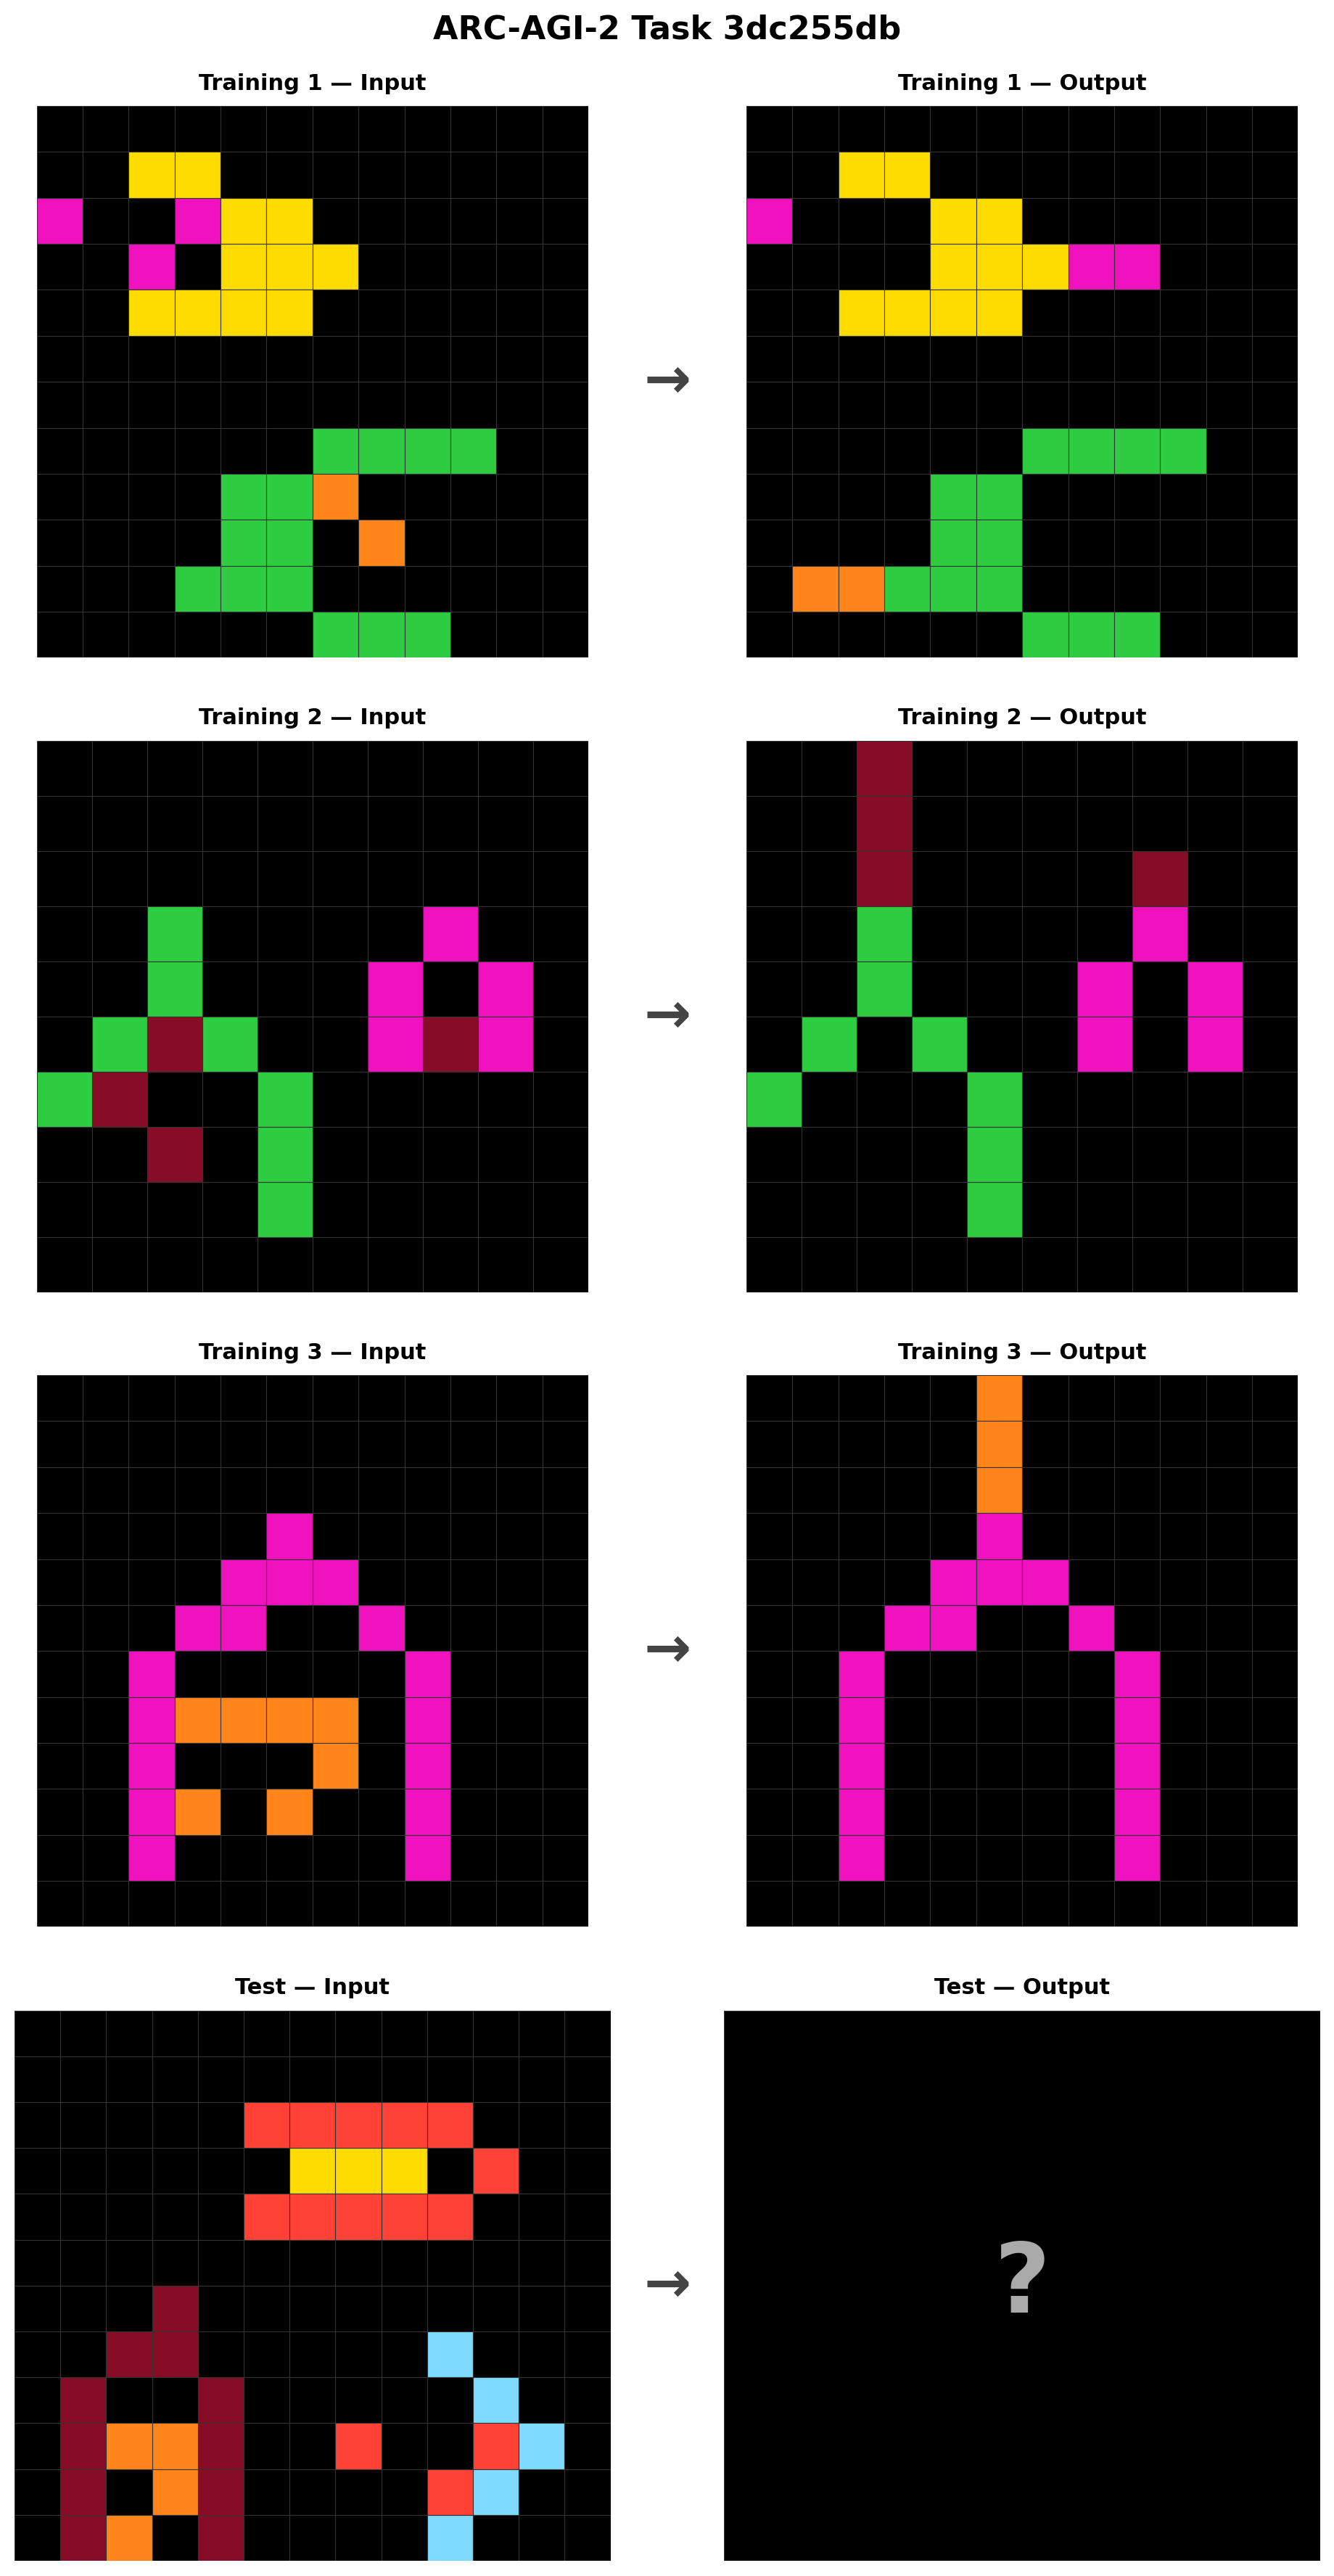
\includegraphics{figures/task_example.png}
\caption{ARC-AGI-2 task \texttt{3dc255db}. A human might see
``spaceships'' with particles on the exhaust side. The transformation
removes the particles from the interior and extends them from the nose.
Three training pairs (rows 1--3) demonstrate the rule; the test input
(row 4) must be solved from these examples alone. This task remains
unsolved by the system.}
\end{figure}

Classical ARC solvers treat tasks as latent programs composed from a
hand-designed DSL (Ferré 2021). Learned approaches attack ARC via
induction or transduction; Li et al. (2025) show that ensembling both
paradigms can approach human-level performance. Test-time adaptation has
emerged as a major axis: Akyürek et al. (2025) demonstrate that updating
model parameters at test time yields strong gains, while Macfarlane and
Bonnet (2025) combine learned representations with explicit program
search.

The broader LLM literature has developed test-time compute techniques
directly relevant to this work. Chain-of-thought prompting (Wei et al.
2022) elicits intermediate reasoning steps; self-consistency (Wang et
al. 2023) samples multiple paths and selects the most common answer.
Tree of Thoughts (Yao, Yu, et al. 2023) reframes inference as search
with branching and backtracking. ReAct (Yao, Zhao, et al. 2023)
interleaves reasoning with tool calls, and PAL (Gao et al. 2023)
translates problems into executable code. Iterative-refinement methods
(Madaan et al. 2023; Shinn et al. 2023) improve outputs through feedback
loops but risk anchoring to early hypotheses. Snell et al. (2025) show
that optimally allocating test-time compute can be more effective than
scaling model parameters.

Relative to this landscape, the present work composes three trends: (i)
hypothesis generation as explicit search across \emph{multiple reasoning
modalities}, extending ToT-style inference (Yao, Yu, et al. 2023); (ii)
tool- and program-mediated reasoning (Yao, Zhao, et al. 2023; Gao et al.
2023) used to produce richer intermediate artifacts for downstream
selection; and (iii) judge-based selection adapted from the
LLM-as-a-judge paradigm (Zheng et al. 2023). What is distinctive is the
combination of heterogeneous candidate generators with
context-preserving comparison over full reasoning traces, rather than
scalar scoring or consensus compression.

\begin{center}\rule{0.5\linewidth}{0.5pt}\end{center}

\hypertarget{method}{%
\section{Method}\label{method}}

The solver is built around a practical observation: to solve tasks that
frontier systems do not already solve, the correct solution is often a
\textbf{minority hypothesis}. If the most common solution were correct,
the task would likely already be within the main cluster of model
behavior. The solver's first phase therefore creates many
\emph{independent} candidate solutions across heterogeneous reasoning
modalities (text, image, and code), maximizing the probability that at
least one candidate captures a genuinely novel hypothesis. Each modality
provides a structurally different representation of the same task, which
empirically produces candidates that cluster differently (Section IV-E).

\hypertarget{pipeline-overview}{%
\subsection{Pipeline Overview}\label{pipeline-overview}}

Fig. 2 shows the end-to-end pipeline. For each ARC task:

\begin{figure}
\centering
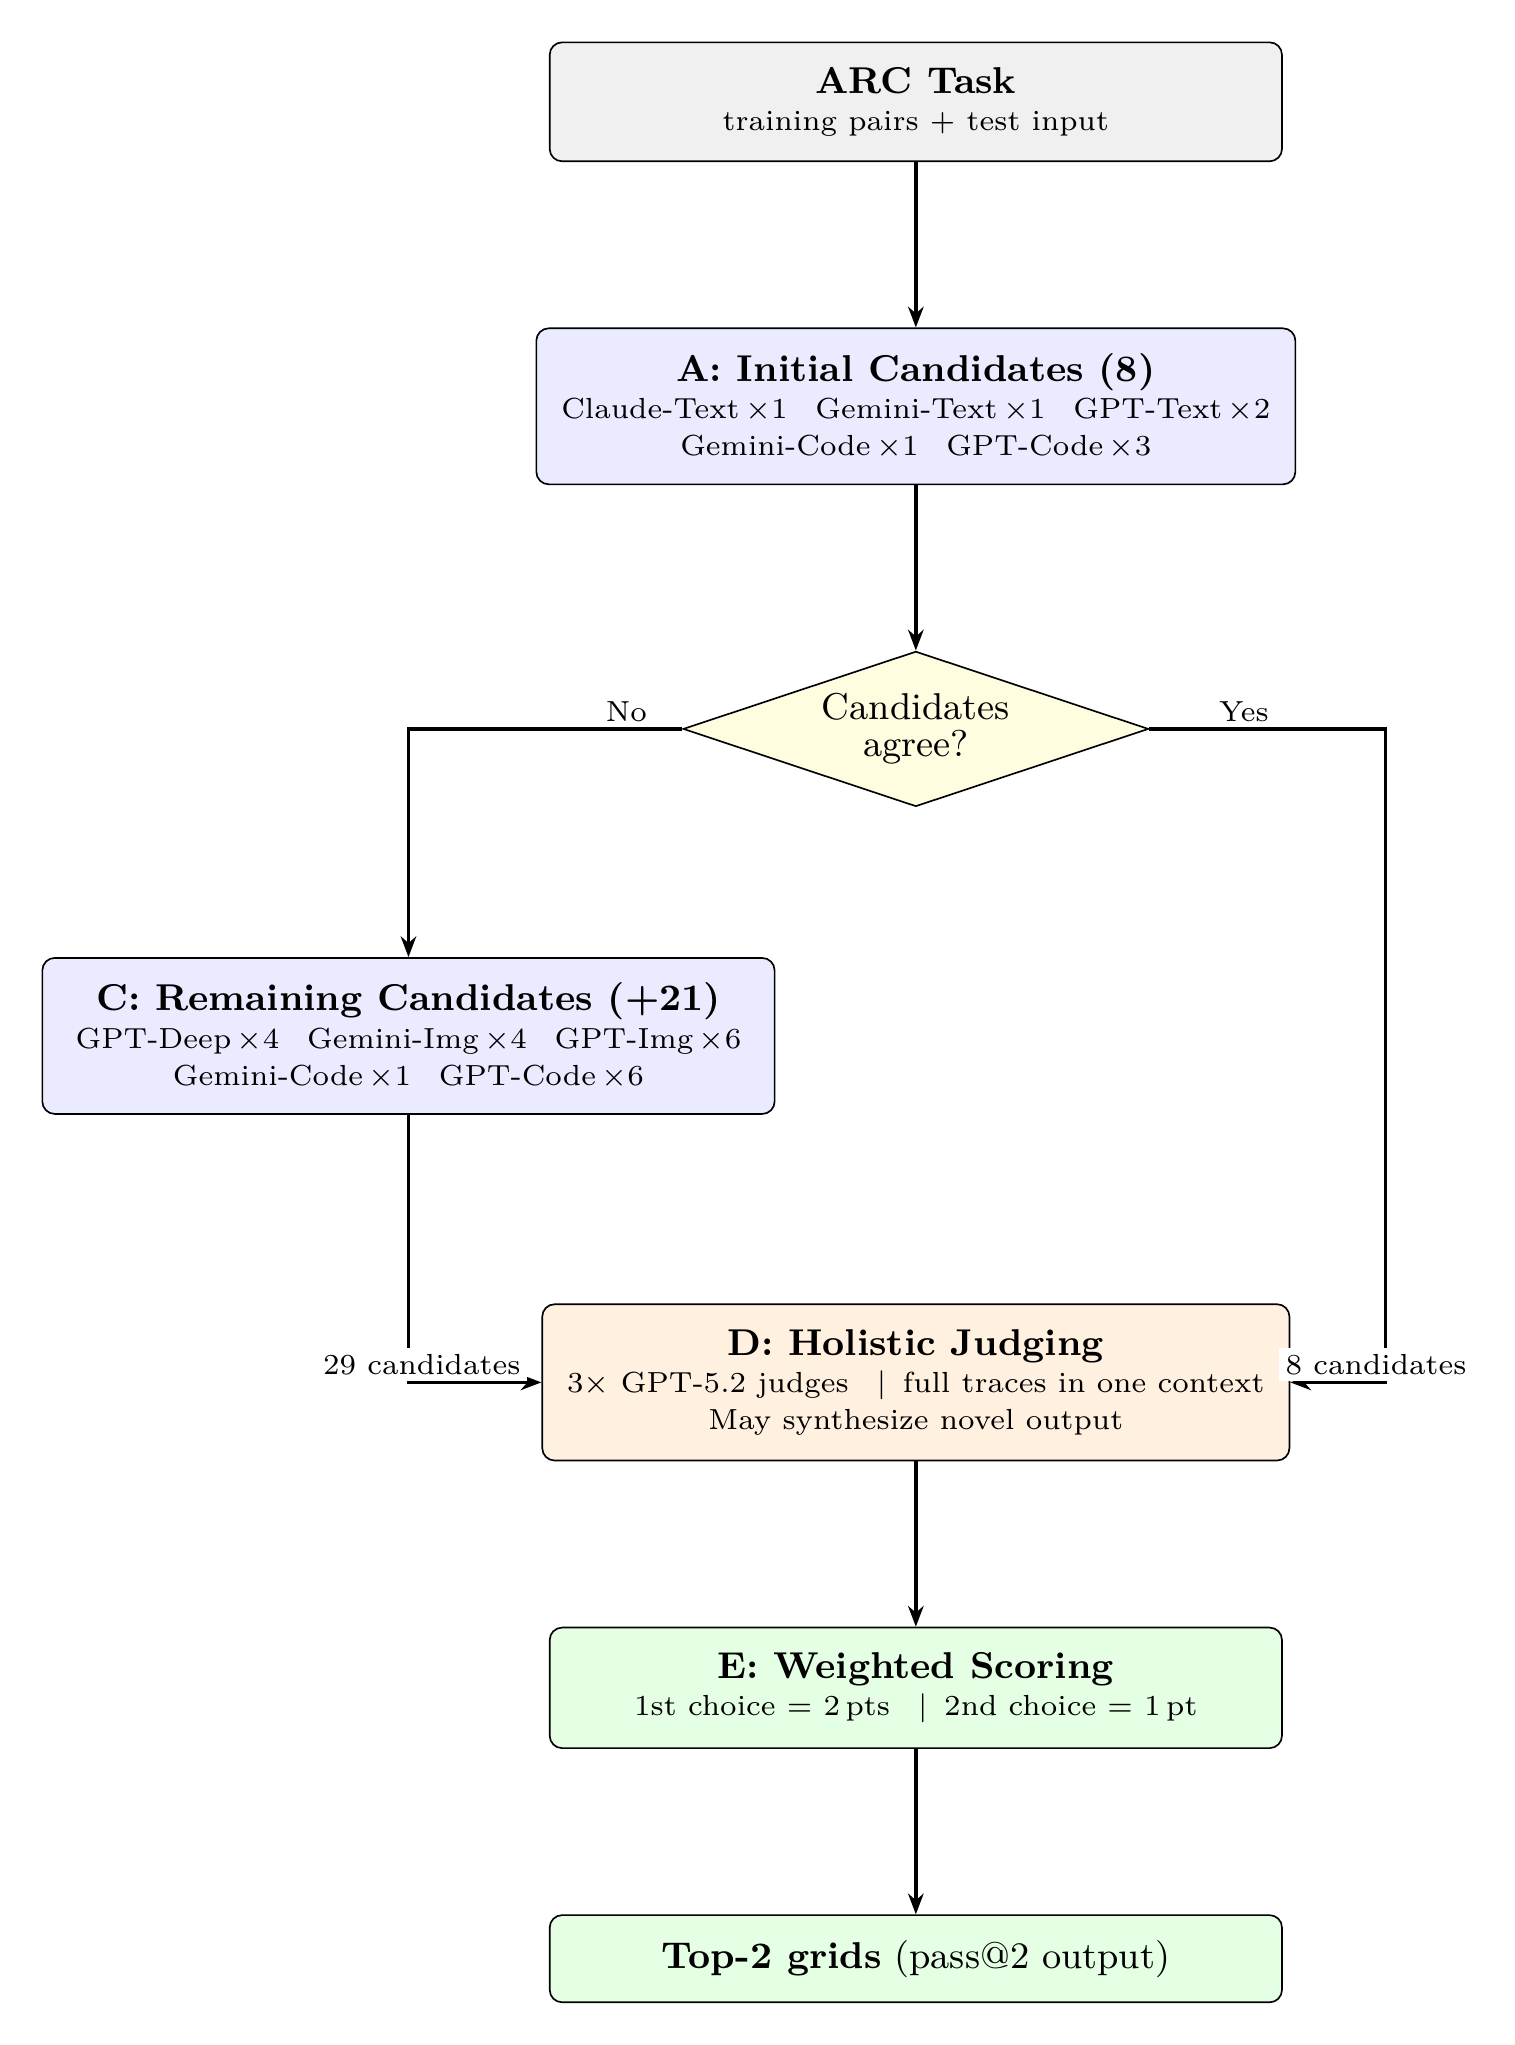
\includegraphics{figures/pipeline.png}
\caption{System pipeline overview.}
\end{figure}

\begin{enumerate}
\def\labelenumi{\arabic{enumi}.}
\item
  \textbf{Candidate generation (up to 29 candidates).} A set of
  modality-specific solvers is run, each producing a single predicted
  output grid, a reasoning trace, and --- for code-generation candidates
  --- the code itself along with tool calls and execution logs. Each
  candidate produces one output; the pass@2 two-guess format is
  introduced only at the judging stage (step 2). Candidate generation
  proceeds in stages: if early-stage candidates already show strong
  agreement (multiple candidates converging on the same output), the
  system terminates early and skips the remaining, more expensive
  modalities. This adaptive early stopping improves cost efficiency on
  tasks that can be solved with a shallower search. On ARC-AGI-1 (which
  contains easier tasks that more frequently trigger early stopping),
  the system achieves 94.5\% on the official semi-private evaluation at
  only \$11.40/task --- substantially cheaper than the \$38.99/task on
  ARC-AGI-2, where harder tasks require the full candidate budget more
  often. Both semi-private scores and costs are as reported by ARC
  Prize's verification infrastructure. On the ARC-AGI-2 public
  evaluation, 37 of 167 instances triggered early stopping (evaluated
  with only 8 candidates instead of 29); of these, \textbf{36 were
  solved correctly} (97.3\% accuracy). The single early-stopping failure
  (\texttt{dbff022c:1}) is a case of extreme groupthink: all models
  confidently assume the simpler of two valid interpretations of a
  legend-to-color mapping, while the ground truth requires the more
  complex one. This validates the heuristic on easy tasks, but also
  illustrates that early consensus can mask genuine ambiguity.
\item
  \textbf{Holistic judging (3 parallel judges).} All candidate traces
  are concatenated into a single long-context prompt. Each judge model
  is asked to identify the top-2 most likely correct candidates (or
  propose a synthesis that recombines correct subcomponents), explain
  why other candidate clusters are wrong, and output the final grids.
\item
  \textbf{Weighted scoring.} Each judge's first choice receives 2 points
  and second choice receives 1 point. The system sums points across
  judges for each distinct output grid. The two grids with the highest
  total score become the solver's pass@2 guesses.
\end{enumerate}

ARC-AGI-2 tasks often introduce new concepts that were not exercised in
the training pairs. A solution can be perfectly ``logical'' on the
training examples but still be a brittle overfit that fails to abstract
the intended rule. This makes naive logic checking of traces
insufficient (Sections III-C and VI). In practice, the system needs
broad hypothesis exploration across structurally different
representations, combined with a judge that can identify \textbf{where}
a candidate is likely overfitting --- even when its reasoning reads as
coherent.

\begin{center}\rule{0.5\linewidth}{0.5pt}\end{center}

\hypertarget{multimodal-candidate-generation}{%
\subsection{Multimodal Candidate
Generation}\label{multimodal-candidate-generation}}

Candidate generation is performed via three foundation models across
multiple inference configurations: \textbf{Gemini 3 Preview} in a
high-reasoning setting (text, image, and code with tools),
\textbf{GPT-5.2} in an x-high reasoning setting (text, image, code with
and without tools, and a deep-think configuration), and \textbf{Claude
Opus 4.5} in a long-context (120k) setting (text reasoning). Exact API
parameters, tool schemas, and prompts are documented in the open-source
implementation. In the final system, generators are grouped into three
families --- \textbf{Text}, \textbf{Image}, and \textbf{Code} --- with
multiple configurations within each family to encourage diversity. Table
1 shows the full candidate configuration.

\textbf{Table 1. Candidate configuration: 29 generators grouped by
family.}

\begin{table}[htbp]
\centering
\footnotesize
\begin{tabular}{@{}lll@{}}
\toprule\noalign{}
Family & Generator & Candidates \\
\midrule\noalign{}

\bottomrule\noalign{}

Text & Claude Opus 4.5 (text) & 1 \\
Text & Gemini 3 Preview (text) & 1 \\
Text & GPT-5.2 (text) & 2 \\
Text & GPT-5.2 (deep think) & 4 \\
Image & Gemini 3 Preview (image) & 4 \\
Image & GPT-5.2 (image) & 6 \\
Code & Gemini 3 Preview (code, tools) & 2 \\
Code & GPT-5.2 (code, tools) & 9 \\
& \textbf{Total} & \textbf{29} \\
\end{tabular}
\end{table}

The text family contributes 8 candidates (including 4 deep-think runs),
image contributes 10, and code contributes 11. Within each family,
multiple runs of the same generator use the same prompt and API
parameters; diversity arises from model sampling stochasticity.

\textbf{Text methodology.} Text candidates are generated by prompting a
language model with a textual encoding of the ARC training pairs and
test input. The model is asked to infer the transformation rule and
output a completed test grid. The base prompt is intentionally minimal:

\begin{Shaded}
\begin{Highlighting}[]
\NormalTok{You are solving an ARC task. Each grid cell is an integer}
\NormalTok{0{-}9 representing a color. Use the solved examples to infer}
\NormalTok{the transformation and apply it to the test input.}
\NormalTok{\{training and test examples\}}
\NormalTok{Respond with an explanation of your thinking ... you MUST}
\NormalTok{also respond with the completed output grid.}
\end{Highlighting}
\end{Shaded}

The prompt deliberately does not prescribe a fixed reasoning template,
step-by-step plan, or output format, which reduces compliance overhead
and empirically increases hypothesis diversity. The trade-off is noisier
outputs that require tolerant parsing and validation to recover
candidate grids (see Section VI for negative results on prescribed
reasoning templates). Grids are encoded in CSV format, selected after
benchmarking multiple representation formats; suboptimal format choices
cost on the order of 10\% lost performance.

\textbf{``Deep think'' variant.} In addition to the standard text
prompt, a ``deep think'' configuration allocates a larger test-time
compute budget by explicitly encouraging GPT-5.2 to reason more
extensively before committing to a final output --- effectively trading
tokens for deeper deliberation within a single response. This accounts
for 4 of the 8 text candidates (Table 1).

\textbf{Image methodology.} Image candidates are generated by rendering
the ARC training pairs and test input as a single annotated image
alongside a textual instruction prompt. This provides the model with a
pixel-space representation that can be advantageous for tasks where
salient structure is more readily perceived visually than through a
textual grid encoding. The image renderings are intentionally
\textbf{imprecise} --- slightly distorted rather than pixel-perfect grid
reproductions. Pixel-perfect renderings underperformed in early
experiments, possibly because models treated them as lossless encodings
and fell back on cell-by-cell numerical reasoning rather than engaging
the visual pattern recognition that makes image prompting valuable. The
slight imprecision appears to encourage models to reason about shapes,
symmetries, and spatial relationships at a higher level of abstraction.
In the public evaluation analysis (Section IV-E), image prompting
provides uniquely correct candidates on several instances.

\textbf{Code methodology.} Code candidates treat ARC solving as program
synthesis: the model is asked to produce executable code that maps input
grids to output grids. Two code-generation regimes are used.
\emph{Tool-integrated code generation} lets the model iteratively write
code, execute it via a sandbox tool, inspect intermediate outputs, and
refine the program across multiple tool calls;\footnote{The ARC Prize
  semi-private evaluation uses OpenAI's zero-data-retention (ZDR) API
  mode, which disables tool calls. For the semi-private run,
  tool-integrated code candidates were replaced with one-shot code
  generation.} this regime often produces rich intermediate artifacts
(program drafts, test harnesses, execution traces) that are later
consumed by the holistic judge. \emph{One-shot code generation} returns
a complete program in a single response without iterative feedback ---
substantially cheaper but less robust on tasks that benefit from
iterative debugging. The tool-integrated regime is the primary code
strategy, contributing the majority of code candidates.

\begin{center}\rule{0.5\linewidth}{0.5pt}\end{center}

\hypertarget{context-preserving-holistic-judging}{%
\subsection{Context-Preserving Holistic
Judging}\label{context-preserving-holistic-judging}}

Given 8--29 candidates per task, many are plausible and internally
coherent. Worse, models tend to \textbf{cluster} around the same wrong
interpretation on the hardest tasks. The key difficulty is identifying a
rare candidate that is correct --- or close enough that it can be
repaired --- without reducing everything to an overly lossy score. Three
judging approaches were tested:

\begin{enumerate}
\def\labelenumi{\arabic{enumi}.}
\tightlist
\item
  \textbf{Logic judge (failed):} Scoring candidates by whether their
  reasoning appears logically consistent fails because a candidate can
  be internally coherent yet overfit to training pairs or miss a latent
  concept introduced in the test case.
\item
  \textbf{Consistency judge (partial):} Selecting themes that repeat
  across candidates rewards the majority cluster, but breaking new
  ground requires elevating \emph{divergent} hypotheses --- the correct
  solution to an unsolved task is often not the modal answer.
\item
  \textbf{Holistic judge (final):} All traces are provided
  \emph{together} in a single prompt, and the judge picks the top-2 most
  likely correct candidates. Three judges run in parallel and their
  picks are aggregated via weighted scoring. This works because having
  all context together beats abstracting traces into scores, letting the
  judge detect subtle but decisive differences between near-identical
  hypotheses.
\end{enumerate}

The holistic judge can be understood as an \textbf{anti-consistency}
mechanism. Self-consistency (Wang et al. 2023) selects the most common
answer across samples --- an effective strategy when the majority is
likely correct. On ARC-AGI-2, the majority is often \emph{wrong} on the
hardest tasks (Section IV-F), making consistency-based selection a
liability. The holistic judge inverts this: it is designed to identify a
correct \emph{minority} hypothesis against a confidently wrong majority,
using full-trace comparison to distinguish genuine insight from
plausible groupthink.

All three judges use \textbf{GPT-5.2} (x-high reasoning setting), the
same model used for candidate generation but in a distinct role with a
different prompt. A mixed-model ensemble (combining Opus, Gemini, and
GPT-5.2) was tested, but three homogeneous GPT-5.2 judges outperformed
the mixed configuration.

\textbf{Judge prompt structure.} The holistic judge prompt is assembled
programmatically and follows this structure (condensed; full
implementation in the open-source release):

\begin{Shaded}
\begin{Highlighting}[]
\NormalTok{Below is a problem attempted \{N\} times:}
\NormalTok{\{training pairs + test input\}}
\NormalTok{\textless{}SOLUTION 1 START\textgreater{}}
\NormalTok{\textless{}CONTENT\textgreater{}\{full reasoning trace\}\textless{}/CONTENT\textgreater{}}
\NormalTok{\textless{}PREDICTED\_GRID\textgreater{}\{candidate output as CSV\}\textless{}/PREDICTED\_GRID\textgreater{}}
\NormalTok{\textless{}SOLUTION 1 STOP\textgreater{}}
\NormalTok{... (repeated for all N solutions) ...}
\NormalTok{Your task is to assess how well they\textquotesingle{}ve understood the}
\NormalTok{problem. Often, new mechanics are introduced in the test}
\NormalTok{example. Please output two solutions that represent the}
\NormalTok{right mechanic for solving the problem.}
\end{Highlighting}
\end{Shaded}

Each candidate's \texttt{CONTENT} block contains the full reasoning
trace --- for text/image candidates this is the model's chain-of-thought
response, and for code candidates it is the complete iterative tool-use
trace including intermediate program drafts, execution outputs, and
debugging steps. Candidates producing identical output grids are listed
as separate solutions with separate traces, preserving the judge's
ability to assess reasoning quality even when outputs agree. The prompt
does \textbf{not} instruct the judge to prefer majority or minority
answers --- it asks for a ``meta-conclusion,'' leaving the judge free to
weigh agreement, reasoning quality, and novelty as it sees fit. The
resulting prompt is intentionally large: on the order of
\textbf{30k--80k input tokens}, making long-context frontier models a
practical requirement for the judge step.

\textbf{Synthesis.} The holistic judge is also permitted to propose a
\textbf{novel solution not identical to any candidate output},
effectively recombining correct subcomponents of multiple flawed
candidates. This matters on tasks where no single candidate fully solves
the problem but multiple candidates contain partial truths. Synthesized
solutions are output as raw grids (not executable code), which means
they do not benefit from programmatic verification and are susceptible
to arithmetic or grid-construction errors.

\textbf{Aggregation.} Each judge outputs a ranked pair of solutions
(first choice and second choice). The system assigns \textbf{2 points}
to each judge's first choice and \textbf{1 point} to each judge's second
choice, then sums points across judges for each distinct output grid.
The two grids with the highest total score become the solver's pass@2
guesses. When judges agree on their top pick, that solution accumulates
up to 6 points; when they disagree, the scoring naturally surfaces the
most broadly supported candidates. A known limitation is that candidate
traces are concatenated in a fixed order without shuffling between judge
runs, which may interact with LLM position biases (Zheng et al. 2023);
shuffling candidate order across runs is a natural improvement.

\begin{center}\rule{0.5\linewidth}{0.5pt}\end{center}

\hypertarget{experiments-and-results}{%
\section{Experiments and Results}\label{experiments-and-results}}

\hypertarget{evaluation-protocol}{%
\subsection{Evaluation Protocol}\label{evaluation-protocol}}

ARC-AGI-2 provides public, semi-private, and private evaluation sets,
all calibrated and scored under \textbf{pass@2} (Chollet et al. 2024).
ARC Prize Verified results are reported on the semi-private evaluation
set via an official verification process and leaderboard. The solver was
iteratively developed using the 1,000-task training set and the 120-task
public evaluation split; the semi-private evaluation was run on held-out
tasks unseen during development, and the \textasciitilde3
percentage-point gap between public and semi-private scores suggests
limited overfitting.

\hypertarget{headline-results}{%
\subsection{Headline Results}\label{headline-results}}

The solver was submitted to the ARC Prize foundation on December 15,
2025, with official results announced on February 3, 2026. The
leaderboard snapshot in Table 2 reflects the state at the time of
announcement.

On the \textbf{semi-private evaluation set}, the solver achieves
\textbf{72.9\% solved} at \textbf{\$38.99/task} -- the highest score on
the ARC Prize Verified leaderboard at the time of writing. On the
\textbf{public evaluation set}, it achieves \textbf{76.11\% solved} at
\textbf{\$19.69/task} (self-measured). For the per-instance analyses
below, the public evaluation split contains 120 task IDs with 167 test
instances (75 tasks with 1 test instance, 43 with 2, and 2 with 3).

The \textasciitilde3 percentage-point gap between public (76.11\%) and
semi-private (72.9\%) likely reflects three factors: (i) natural
generalization loss to a held-out task distribution, (ii) the
semi-private verification uses OpenAI's zero-data-retention (ZDR) API
mode, which disables function/tool calling, and (iii) the semi-private
run coincided with a period of known instability in OpenAI's API. Under
ZDR, the tool-integrated code generation candidates (Section III-B) were
replaced with one-shot code generation without iterative sandbox
execution. Code candidates were still produced, but without the
iterative debugging loop that makes tool-integrated generation more
robust on complex tasks. Since tool-integrated code generation accounts
for the bulk of the Code family's cost (Table 7), the ZDR constraint
both reduced accuracy and changed the cost profile of the semi-private
run relative to the public run.

\textbf{Table 2. Leaderboard snapshot and reference systems.}\footnote{https://arcprize.org/leaderboard}
Semi-private results are as reported on the ARC Prize Verified
leaderboard at the time of the official results announcement (February
3, 2026); the public-evaluation row is self-measured.

\begin{table}[htbp]
\centering
\footnotesize
\begin{tabular}{@{}
  >{\raggedright\arraybackslash}p{(\columnwidth - 8\tabcolsep) * \real{0.2000}}
  >{\raggedright\arraybackslash}p{(\columnwidth - 8\tabcolsep) * \real{0.2000}}
  >{\raggedright\arraybackslash}p{(\columnwidth - 8\tabcolsep) * \real{0.2000}}
  >{\raggedright\arraybackslash}p{(\columnwidth - 8\tabcolsep) * \real{0.2000}}
  >{\raggedright\arraybackslash}p{(\columnwidth - 8\tabcolsep) * \real{0.2000}}@{}}
\toprule\noalign{}
\begin{minipage}[b]{\linewidth}\raggedright
AI System
\end{minipage} & \begin{minipage}[b]{\linewidth}\raggedright
Author
\end{minipage} & \begin{minipage}[b]{\linewidth}\raggedright
ARC-AGI-2
\end{minipage} & \begin{minipage}[b]{\linewidth}\raggedright
Cost/Task
\end{minipage} & \begin{minipage}[b]{\linewidth}\raggedright
Comment
\end{minipage} \\
\midrule\noalign{}

\bottomrule\noalign{}

Human Panel & Human & 100.00\% & \$17.00 & At least two humans out of
\textasciitilde400 solved it \\
This paper & Johan Land & 72.90\% & \$38.99 & Semi-private (official) \\
This paper & Johan Land & 76.11\% & \$19.69 & Public eval \\
GPT-5.2 Pro (High) & OpenAI & 54.20\% & \$15.72 & \\
Gemini 3 Pro (Refine.) & Poetiq & 54.00\% & \$30.57 & \\
GPT-5.2 (X-High) & OpenAI & 52.90\% & \$1.90 & \\
Gemini 3 Deep Think (Preview) & Google & 45.10\% & \$77.16 & \\
GPT-5.2 (High) & OpenAI & 43.30\% & \$1.39 & \\
GPT-5.2 Pro (Medium) & OpenAI & 38.50\% & \$8.99 & \\
Opus 4.5 (Thinking, 64K) & Anthropic & 37.60\% & \$2.40 & \\
Gemini 3 Flash Preview (High) & Google & 33.60\% & \$0.23 & \\
\end{tabular}
\end{table}

The system achieves +18.7 percentage points over the strongest
commercial baselines at higher cost, reflecting additional test-time
compute spent on multi-candidate search. The remaining gap to the human
panel (100.0\% at \$17/task) indicates substantial headroom. As the
leaderboard evolves rapidly, the contribution is the
\textbf{architectural pattern} rather than the specific accuracy
numbers.

\hypertarget{efficiency}{%
\subsection{Efficiency}\label{efficiency}}

ARC-AGI-2 explicitly evaluates efficiency (Chollet et al. 2024). The
roughly 2x cost difference between the semi-private and public runs
(\$38.99 vs.~\$19.69) is largely attributable to API-level
unreliability: on the public-eval run, only 2,216 of 14,106 GPT-5.2 API
attempts succeeded (84\% failure rate due to rate limits, timeouts, and
server errors). The public-eval cost of \$19.69/task is a more
representative measure; at this cost, the solver is comparable to
GPT-5.2 Pro (\$15.72/task) while achieving a +21.9 percentage-point
accuracy gain, and is both cheaper and more accurate than Gemini 3 Pro
(\$30.57/task at 54.0\%). A detailed cost breakdown is provided in
Section V.

\hypertarget{modality-contribution}{%
\subsection{Modality Contribution}\label{modality-contribution}}

The final modality mix was selected based on two criteria: raw solve
contribution and diversity contribution (uniquely solved tasks that
other modalities fail). GPT dominates code generation, with Gemini
adding meaningful diversity; for image reasoning, Gemini and GPT behave
differently and are complementary; Opus is exceptional for end-to-end
text reasoning, being the sole solver for several tasks via text-only
reasoning. Over the 167 public-evaluation test instances, the final
system solves 128/167 = 76.65\% at the instance level (pass@2). The
candidate pool contains at least one correct output for 144/167 =
86.23\% of instances (candidate-oracle accuracy). The 39 unsolved
instances decompose into 21/167 generation failures where no candidate
in the pool is correct (with full 29-candidate coverage), 1/167
early-stopping failure where consensus among the initial 8 candidates
was incorrect (Section III), and 17/167 selection failures where at
least one correct candidate exists but is not chosen by the judge.
Notably, there is one instance where the final output is correct despite
\textbf{zero} candidates matching ground truth (\texttt{21897d95:2});
this occurs via judge synthesis (Section IV-F). Generation failures tend
to involve long chains of dependent reasoning steps where all candidates
make errors at different points in the chain; selection failures cluster
around cases where the test instance introduces a new mechanic not fully
disambiguated by training examples, creating genuine ambiguity that the
judge cannot resolve.

\begin{figure}
\centering

\includegraphics{figures/methodology_matrix.png}
\caption{Methodology matrix over public evaluation instances. Green =
candidate matches ground truth; red = candidate does not match; white =
candidate not produced (early stopping). Rows are test instances;
columns are candidate generators grouped by modality family.}
\end{figure}

\hypertarget{modality-complementarity-public-eval}{%
\subsection{Modality Complementarity (Public
Eval)}\label{modality-complementarity-public-eval}}

To quantify complementarity between candidate-generation methodologies,
I evaluate each candidate output against ground truth and record a
per-instance correctness matrix. To avoid conflating uniqueness with
conditional execution (the system uses adaptive early stopping for easy
tasks), the analysis is restricted to the 130 instances with complete
candidate coverage (all 29 candidates generated).

\textbf{Table 3. Pairwise non-overlap between modality families (n =
130).} Each cell reads ``row solves, column does not'': the entry counts
instances with at least one PASS in the row family and zero PASS in the
column family. The table is not symmetric.

\begin{table}[htbp]
\centering
\footnotesize
\begin{tabular}{@{}llll@{}}
\toprule\noalign{}
& Text & Image & Code \\
\midrule\noalign{}

\bottomrule\noalign{}

Text & NA & 13 & 7 \\
Image & 17 & NA & 11 \\
Code & 18 & 18 & NA \\
\end{tabular}
\end{table}

Each family covers a non-trivial set of instances that are not covered
by at least one other family. At the exclusive level, 2 instances are
solved only by Text, 6 only by Image, and 7 only by Code. This confirms
that modalities function as distinct search operators rather than
redundant copies of the same reasoning process, and supports treating
each modality as a separate exploration channel in the
candidate-generation phase.

\hypertarget{judging-and-synthesis-public-eval}{%
\subsection{Judging and Synthesis (Public
Eval)}\label{judging-and-synthesis-public-eval}}

Holistic judging (excluding synthesis) yielded a net uplift of
\textbf{+7 solved instances} relative to a majority-vote baseline that
selects the most common candidate output. All 7 are minority recoveries
-- cases where the correct answer was not the most frequent candidate
output and the holistic judge identified it by reasoning over full
traces rather than counting votes. This directly validates the
anti-consistency motivation: on these tasks the majority cluster was
wrong, and the judge's ability to read and compare reasoning traces was
the deciding factor. One illustrative case is \texttt{dfadab01:1}, where
12 candidates converge on one incorrect output and 8 on another, but the
judge identifies the lone correct candidate. The judge rationale shows
explicit anti-consistency reasoning:

\begin{Shaded}
\begin{Highlighting}[]
\NormalTok{Most candidate solvers correctly identify the core stamp}
\NormalTok{mechanic ... The only remaining ambiguity is edge handling}
\NormalTok{(not clearly disambiguated by the training set):}
\NormalTok{{-} Some solvers assume a stamp must fit fully.}
\NormalTok{{-} Others assume stamps are clipped at the border.}
\NormalTok{So the two most plausible outputs (same mechanic,}
\NormalTok{differing only in border handling)}
\end{Highlighting}
\end{Shaded}

Rather than committing both guesses to the majority interpretation, the
judge uses the pass@2 format to hedge across the two edge-handling
interpretations --- reasoning that majority voting cannot perform.

Synthesis -- where the judge produces a novel output not identical to
any candidate -- yielded \textbf{+1 additional solved instance}
(\texttt{21897d95:2}), a task where none of the 29 candidates were
correct but the judge recombined partial insights (correct room parsing
from some candidates, correct arrow semantics from others) into a novel
correct output.

\begin{center}\rule{0.5\linewidth}{0.5pt}\end{center}

\hypertarget{ablation-studies}{%
\section{Ablation Studies}\label{ablation-studies}}

A rigorous component attribution would require multiple full-pipeline
runs with individual components removed or substituted. Each such run
costs approximately \$2,400 in API spend (Table 6), making extensive
ablation prohibitively expensive. This paper therefore relies primarily
on \textbf{post-hoc analysis of the single public evaluation run},
extracting what can be measured from the existing candidate pool rather
than running dedicated ablation experiments. This approach has clear
limitations: it cannot capture interaction effects between components,
and some comparisons (e.g., end-to-end modality removal) require fresh
runs that have not been performed. Unless otherwise stated, ``solved''
refers to pass@2 at the \textbf{test-instance} level on the public
evaluation split (167 instances).

\hypertarget{measured-ablations}{%
\subsection{Measured Ablations}\label{measured-ablations}}

\textbf{Table 5. Measured judge ablations on the public evaluation run.}
Reported deltas are net solved-instance uplifts attributable to the
indicated component.

\begin{table}[htbp]
\centering
\footnotesize
\begin{tabular}{@{}
  >{\raggedright\arraybackslash}p{(\columnwidth - 4\tabcolsep) * \real{0.3333}}
  >{\raggedright\arraybackslash}p{(\columnwidth - 4\tabcolsep) * \real{0.3333}}
  >{\raggedright\arraybackslash}p{(\columnwidth - 4\tabcolsep) * \real{0.3333}}@{}}
\toprule\noalign{}
\begin{minipage}[b]{\linewidth}\raggedright
Component
\end{minipage} & \begin{minipage}[b]{\linewidth}\raggedright
Ablation / control condition
\end{minipage} & \begin{minipage}[b]{\linewidth}\raggedright
Net uplift (solved instances)
\end{minipage} \\
\midrule\noalign{}

\bottomrule\noalign{}

Holistic selection & Holistic judge vs majority-vote baseline (synthesis
disabled in both) & +7 (all minority recoveries) \\
Judge synthesis & Synthesis enabled vs disabled (holistic selection held
fixed) & +1 \\
\end{tabular}
\end{table}

The +7 holistic selection uplift directly validates the anti-consistency
design: all 7 gains are minority recoveries where the correct answer was
not the most frequent candidate output, and the judge's ability to read
and compare full reasoning traces -- rather than simply tallying outputs
-- was the deciding factor. Synthesis yielded +1 instance where no
candidate was correct but the judge recombined partial insights from
complementary failures into a novel correct output. While the measured
synthesis uplift is small on this run, the mechanism has particular
potential on harder tasks where no single candidate is fully correct but
multiple candidates contain complementary partial insights.

\hypertarget{cost-attribution}{%
\subsection{Cost Attribution}\label{cost-attribution}}

\textbf{Table 6. Cost attribution per test instance on the public
evaluation run (n = 167).}

\begin{table}[htbp]
\centering
\footnotesize
\begin{tabular}{@{}llll@{}}
\toprule\noalign{}
Phase & Total (\$) & Avg \$/instance & \% of total \\
\midrule\noalign{}

\bottomrule\noalign{}

Candidate generation & 2081.37 & 12.46 & 87.1\% \\
Judging & 308.91 & 1.85 & 12.9\% \\
\textbf{Total} & \textbf{2390.28} & \textbf{14.31} & \textbf{100\%} \\
\end{tabular}
\end{table}

\textbf{Table 7. Candidate generation cost by modality family.}

\begin{table}[htbp]
\centering
\footnotesize
\begin{tabular}{@{}llll@{}}
\toprule\noalign{}
Modality family & Total (\$) & Avg \$/instance & \% of generation
cost \\
\midrule\noalign{}

\bottomrule\noalign{}

Text (incl.~deep think) & 597.70 & 3.58 & 28.7\% \\
Image & 467.10 & 2.80 & 22.5\% \\
Code & 1016.56 & 6.09 & 48.9\% \\
\end{tabular}
\end{table}

Candidate generation dominates at 87\% of spend; code is the most
expensive family (49\% of generation cost) due to iterative sandbox
execution. Judging contributes +7 solved instances (holistic selection)
and +1 (synthesis) at only 13\% of total cost, making it highly
cost-effective.

\hypertarget{unperformed-ablations}{%
\subsection{Unperformed Ablations}\label{unperformed-ablations}}

The following ablations would strengthen the paper's claims but have not
been run due to cost constraints (\textasciitilde\$2,400 per full run).
They are listed as transparency about what remains unknown and as a
roadmap for future work:

\begin{itemize}
\tightlist
\item
  \textbf{End-to-end modality removal:} run the full pipeline with one
  modality family removed and re-run judging on the reduced candidate
  pool, capturing interaction effects not visible in oracle-level
  analysis.
\item
  \textbf{Candidate budget scaling:} sweep the number of candidates per
  modality to estimate marginal returns and identify diminishing-returns
  regimes.
\item
  \textbf{Trace content ablation:} compare judge accuracy with full
  reasoning traces vs output grids only, to quantify whether trace
  content actually helps selection or whether the judge primarily relies
  on output comparison.
\end{itemize}

\begin{center}\rule{0.5\linewidth}{0.5pt}\end{center}

\hypertarget{negative-results}{%
\section{Negative Results}\label{negative-results}}

This section documents approaches explored during development that were
ultimately discarded, often because they reduced diversity, increased
brittleness, or forced premature abstraction. Two findings stand out for
their direct impact on the final system design.

\textbf{Prescriptive prompting degrades performance.} Perhaps the most
counterintuitive finding is that extensive prompt engineering --
prescribed reasoning templates, structured output requirements,
chain-of-thought scaffolding, domain-specific heuristics -- consistently
hurt performance on the hardest tasks. The mechanism appears to be a
\textbf{compliance tax on reasoning}: when instructed \emph{how} to
think, the model allocates a significant portion of its reasoning budget
to following instructions rather than solving the problem. On easy tasks
this overhead is harmless, but on hard tasks where creative leaps are
required, the model dutifully follows the prescribed template and never
explores the unstructured reasoning path that might have led to the
correct solution. Prescriptive prompts also interact with diversity:
when all N candidates follow the same reasoning template, they tend to
converge on the same (possibly wrong) answer. A minimal prompt allows
different candidates to approach the problem from genuinely different
angles. The final system uses deliberately minimal prompts with no
prescribed structure, tolerating noisy outputs with robust downstream
parsing.

\textbf{Hint generation collapsed diversity.} A two-stage approach --
generate a hint, then solve conditioned on the hint, structurally
similar to Self-Refine (Madaan et al. 2023) and Reflexion (Shinn et al.
2023) -- was tested and discarded. The hint stage consistently narrowed
candidate diversity into a smaller hypothesis space, which is
counterproductive when the correct solution may require an
unconventional reasoning path. Similarly, structured decomposition
(object identification followed by transformation identification
followed by solving) suffered from brittle stage handoffs that regressed
candidate outputs toward the mean rather than expanding the hypothesis
space.

Several other approaches were also discarded: Opus codegen and image
reasoning contributed less uniquely than GPT/Gemini configurations and
were dropped from the final mix; forcing strict output schemas (e.g.,
JSON via API-level response format constraints) underperformed free-form
output with robust parsing; and synthetic data augmentation for code
candidates (color permutation, rotation, mirroring) added no meaningful
signal because surface-level augmentations do not test new structural
properties and geometric transforms can break task semantics for
orientation-dependent tasks.

\begin{center}\rule{0.5\linewidth}{0.5pt}\end{center}

\hypertarget{discussion-and-conclusion}{%
\section{Discussion and Conclusion}\label{discussion-and-conclusion}}

This paper demonstrates that strong ARC-AGI-2 performance can be
achieved by treating \textbf{modalities as search operators} --
generating candidates independently across heterogeneous reasoning
channels (text, image, code) to maximize hypothesis diversity, then
selecting using holistic judging over full traces. At the time of
writing, this approach achieves the highest score on the ARC Prize
Verified leaderboard (72.9\%), surpassing the best-performing standalone
frontier models -- GPT-5.2 Pro (54.2\%) and Gemini 3 Pro (54.0\%) -- by
+18.7 percentage points. This substantial margin suggests that
orchestrating diverse reasoning modalities with principled selection is
a more effective strategy for abstract reasoning than scaling any single
model alone.

The system's core contributions are architectural rather than
model-specific. First, multi-modal candidate generation exploits the
observation that text, image, and code representations activate
different reasoning pathways -- each modality exclusively solves tasks
inaccessible to the others (Table 3). Second, holistic judging over full
reasoning traces recovers minority-correct solutions that majority
voting discards, yielding +7 instances of uplift. Third, judge synthesis
enables the construction of novel correct outputs from complementary
partial insights when no single candidate is fully correct. These
mechanisms are complementary: diverse generation expands the hypothesis
space, while context-preserving selection navigates it.

\hypertarget{limitations}{%
\subsection{Limitations}\label{limitations}}

\textbf{Cost and practical scalability.} The system spends
\$19.69--\$38.99 per task -- orders of magnitude more expensive than a
single model call. ARC Prize explicitly treats efficiency as a
first-class metric (Chollet et al. 2024), and the current system is far
from efficient. The brute-force strategy of generating 29 candidates
across three models and three modalities, then running three separate
judge passes, is effective but wasteful; a production system would need
adaptive routing that allocates expensive modalities only when
uncertainty is high, but no such mechanism has been developed here.

\textbf{Single-run results.} The headline numbers (76.11\% public,
72.9\% semi-private) each come from a single evaluation run. LLM outputs
are stochastic, and the system's reliance on sampling diversity means
that results will vary across runs; no confidence intervals are reported
because repeated full-pipeline runs were not performed (each costing
\textasciitilde\$2,400).

\textbf{No learning across tasks.} The system treats each task
independently --- no information is carried from one task to the next,
unlike a human solver who would build intuitions across tasks.

\textbf{Narrow evaluation domain.} The system has been evaluated
exclusively on ARC-AGI-2; whether the architectural pattern ---
modality-driven search with holistic judging --- generalizes to other
abstract reasoning benchmarks or broader AI tasks is unknown.

\textbf{Reproducibility fragility.} The system depends on specific
proprietary model snapshots (GPT-5.2, Gemini 3 Preview, Opus 4.5) and
vendor-specific reasoning settings that may change or become unavailable
over time. Results may not be exactly reproducible even with identical
prompts and parameters if the underlying model versions
drift.\footnote{Source code: https://github.com/beetree/ARC-AGI.
  Complete raw data for the public evaluation run (prompts, responses,
  reasoning traces, judge transcripts; over 7 million lines):
  https://www.kaggle.com/code/johanland/johan-land-solver-v7-public/comments?scriptVersionId=290052212.}

\hypertarget{future-directions}{%
\subsection{Future Directions}\label{future-directions}}

Two directions appear most promising. \textbf{Adaptive routing} would
allocate expensive modalities only when early-stage candidates show low
agreement, reducing cost without sacrificing accuracy on hard tasks; the
early-stopping heuristic already demonstrates the principle (97.3\%
accuracy on easy tasks at reduced cost), but a more principled
uncertainty-driven routing mechanism could extend this to the full
difficulty spectrum. \textbf{Synthesis gating} would trigger judge
synthesis only when candidate agreement is low or when multiple
candidates contain complementary partial solutions, potentially
amplifying the +1 instance uplift observed in this work on harder tasks
where the recombination mechanism has the most potential.

\hypertarget{acknowledgments}{%
\subsection{Acknowledgments}\label{acknowledgments}}

Thank you to the ARC-AGI Discord community for valuable discussion and
shared insights throughout the development of this work, and to Greg
Kamradt at ARC Prize for conducting the official semi-private
evaluation.

\hypertarget{refs}{}
\begin{CSLReferences}{1}{0}
\leavevmode\vadjust pre{\hypertarget{ref-akyurek2024surprising}{}}%
Akyürek, Ekin, Mehul Damani, Adam Zweiger, Linlu Qiu, Han Guo, Jyothish
Pari, Yoon Kim, and Jacob Andreas. 2025. {``The Surprising Effectiveness
of Test-Time Training for Few-Shot Learning.''} In \emph{Proceedings of
the 42nd International Conference on Machine Learning}, 267:942--63.
PMLR.

\leavevmode\vadjust pre{\hypertarget{ref-chollet2019measure}{}}%
Chollet, François. 2019. {``On the Measure of Intelligence.''}
\emph{arXiv Preprint arXiv:1911.01547}.

\leavevmode\vadjust pre{\hypertarget{ref-arcprize2024report}{}}%
Chollet, François, Mike Knoop, Gregory Kamradt, and Bryan Landers. 2024.
{``{ARC Prize 2024}: Technical Report.''} \emph{arXiv Preprint
arXiv:2412.04604}.

\leavevmode\vadjust pre{\hypertarget{ref-ferre2021arc}{}}%
Ferré, Sébastien. 2021. {``First Steps of an Approach to the {ARC}
Challenge Based on Descriptive Grid Models and the Minimum Description
Length Principle.''} \emph{arXiv Preprint arXiv:2112.00848}.

\leavevmode\vadjust pre{\hypertarget{ref-gao2023pal}{}}%
Gao, Luyu, Aman Madaan, Shuyan Zhou, Uri Alon, Pengfei Liu, Yiming Yang,
Jamie Callan, and Graham Neubig. 2023. {``{PAL}: Program-Aided Language
Models.''} \emph{International Conference on Machine Learning}.

\leavevmode\vadjust pre{\hypertarget{ref-land2026modality}{}}%
Land, Johan. 2026. {``Modality-Driven Search with Holistic Trace Judging
for {ARC-AGI-2}.''} \emph{arXiv Preprint}.

\leavevmode\vadjust pre{\hypertarget{ref-li2024induction}{}}%
Li, Wen-Ding, Keya Hu, Carter Larsen, Yuqing Wu, Simon Alford, Caleb
Woo, Spencer M. Dunn, et al. 2025. {``Combining Induction and
Transduction for Abstract Reasoning.''} In \emph{International
Conference on Learning Representations}.

\leavevmode\vadjust pre{\hypertarget{ref-bonnet2024latent}{}}%
Macfarlane, Matthew V., and Clément Bonnet. 2025. {``Searching Latent
Program Spaces.''} In \emph{Advances in Neural Information Processing
Systems}. Vol. 38.

\leavevmode\vadjust pre{\hypertarget{ref-madaan2023selfrefine}{}}%
Madaan, Aman, Niket Tandon, Prakhar Gupta, Skyler Hallinan, Luyu Gao,
Sarah Wiegreffe, Uri Alon, et al. 2023. {``Self-Refine: Iterative
Refinement with Self-Feedback.''} \emph{Advances in Neural Information
Processing Systems} 36.

\leavevmode\vadjust pre{\hypertarget{ref-shinn2023reflexion}{}}%
Shinn, Noah, Federico Cassano, Ashwin Gopinath, Karthik Narasimhan, and
Shunyu Yao. 2023. {``Reflexion: Language Agents with Verbal
Reinforcement Learning.''} \emph{Advances in Neural Information
Processing Systems} 36.

\leavevmode\vadjust pre{\hypertarget{ref-snell2024scaling}{}}%
Snell, Charlie, Jaehoon Lee, Kelvin Xu, and Aviral Kumar. 2025.
{``Scaling {LLM} Test-Time Compute Optimally Can Be More Effective Than
Scaling Model Parameters.''} In \emph{International Conference on
Learning Representations}.

\leavevmode\vadjust pre{\hypertarget{ref-wang2022selfconsistency}{}}%
Wang, Xuezhi, Jason Wei, Dale Schuurmans, Quoc Le, Ed Chi, Sharan
Narang, Aakanksha Chowdhery, and Denny Zhou. 2023. {``Self-Consistency
Improves Chain of Thought Reasoning in Language Models.''} In
\emph{International Conference on Learning Representations}.

\leavevmode\vadjust pre{\hypertarget{ref-wei2022chain}{}}%
Wei, Jason, Xuezhi Wang, Dale Schuurmans, Maarten Bosma, Brian Ichter,
Fei Xia, Ed Chi, Quoc Le, and Denny Zhou. 2022. {``Chain-of-Thought
Prompting Elicits Reasoning in Large Language Models.''} \emph{Advances
in Neural Information Processing Systems} 35.

\leavevmode\vadjust pre{\hypertarget{ref-yao2023tree}{}}%
Yao, Shunyu, Dian Yu, Jeffrey Zhao, Izhak Shafran, Thomas L. Griffiths,
Yuan Cao, and Karthik Narasimhan. 2023. {``Tree of Thoughts: Deliberate
Problem Solving with Large Language Models.''} In \emph{Advances in
Neural Information Processing Systems}. Vol. 36.

\leavevmode\vadjust pre{\hypertarget{ref-yao2022react}{}}%
Yao, Shunyu, Jeffrey Zhao, Dian Yu, Nan Du, Izhak Shafran, Karthik
Narasimhan, and Yuan Cao. 2023. {``{ReAct}: Synergizing Reasoning and
Acting in Language Models.''} \emph{International Conference on Learning
Representations}.

\leavevmode\vadjust pre{\hypertarget{ref-zheng2023judging}{}}%
Zheng, Lianmin, Wei-Lin Chiang, Ying Sheng, Siyuan Zhuang, Zhanghao Wu,
Yonghao Zhuang, Zi Lin, et al. 2023. {``Judging {LLM}-as-a-Judge with
{MT-Bench} and {Chatbot Arena}.''} \emph{Advances in Neural Information
Processing Systems} 36.

\end{CSLReferences}

\end{document}
